\documentclass[11pt]{report}
\usepackage{mathtools, amsthm, mathpazo, epic, eepic, color, paralist}
\usepackage{tikz}
\usepackage[margin=1in]{geometry}

\newcommand{\typo}[4]{\item Typo: on line #2 of page #1: \emph{#3} should be \emph{#4}.}
\newcommand{\funcleft}[2]{\item Example #1 on page #2.}


\begin{document}

\chapter*{APEX Section 5.3 Changes}

{\slshape Note: throughout, a positive line number refers to a line that far from the top of the page, a negative line number refers to a line that far from the bottom of the page.}

\section*{Text}

\begin{enumerate}

\item There should be a paragraph break between lines 14 and 15 on page 211.

\item Mimicking what the text does for integral notation on page 190, we should insert the following after line 4 on page 212:

\emph{ \[\sum_{i=1}^9 a_i\] Lets analyze this notation.}

\item Insert the following note after Theorem 37:

{\slshape Note: In practice we will sometimes need variations on formulas 5, 6, and 7 above. For example, we note that \[\sum_{i=0}^n i=0+1+2+\cdots+n=0+\sum_{i=1}^n i=0+\frac{n(n+1)}{2}=\frac{n(n+1)}{2}\text{,}\] so we see that \[\sum_{i=0}^n i=\frac{n(n+1)}{2}.\] Similarly, we find that 
\begin{equation*}
\begin{split}
\sum_{i=0}^n i^2&=\frac{n(n+1)(2n+1)}{6}\text,{\quad and}\\
\sum_{i=0}^n i^3&=\left(\frac{n(n+1)}{2}\right)^2\\
\end{split}
\end{equation*}
}

\item The solution to Example 120 (page 213) should include justifications, i.e.
\begin{equation*}
\begin{split}
\sum_{i=1}^6 (2i-1)&=\sum_{i=1}^6 2i-\sum_{i=1}^6 (1) \quad \text{(Theorem 37(2))}\\
&=\left( 2\sum_{i=1}^6 i\right) -\sum_{i=1}^6 (1) \quad \text{(Theorem 37(3))}\\
&=2\left(\frac{6(6+1)}{2}\right)-6\quad \text{(Theorem 37(1,5))}\\
&=2(21)-6=36\\
\end{split}
\end{equation*}

\item Reindexing Riemann sums. 
\begin{enumerate}
\item The subscripts in Figure 5.17 should each be reduced by 1.

\item Beginning with the second paragraph after the subsection heading {\bfseries Riemann Sums}, change the text to read as follows:

{\slshape Figure 5.17 shows a number line of $[0,4]$ subdivided into 16 equally spaced subintervals. We denote $0$ as $x_0$; we have marked the values of $x_4$, $x_8$, $x_{12}$, and $x_{16}$. We could mark them all, but the figure would get crowded. While it is easy to figure that $x_9=2.25$, in general, we want a method of determining the value of $x_i$ without consulting the figure. Consider:}

\item In the displayed equation immediately following the above text, $x_1$ should be replaced with $x_0$ in both instances.

\item Line -5 on page 214 should read \emph{So $x_9=x_0+9(4/16)=9/4=2.25$.}

\item In lines -3 \& -2 on page 214, change to read \emph{We could compute $x_{31}$ as \[x_{31}=x_0+31(4/100)=124/100=1.24.\]}

\item At the top of page 215, it should read {\slshape Given any subdivision of $[0,4]$, the first subinterval is $[x_0,x_1]$; the second is $[x_1,x_2]$; the $i^{th}$ subinterval is $[x_{i-1},x_i]$.

When using the Left Hand Rule, the height of the $i^{th}$ rectangle will be $f(x_{i-1})$.

When using the Right Hand Rule, the height of the $i^{th}$ rectangle will be $f(x_i)$.

When using the Midpoint Rule, the height of the $i^{th}$ rectangle will be $f\left(\frac{x_{i-1}+x_i}{2}\right)$.}

\item The indexing on the Left Hand, Right Hand, and Midpoint Rules at the top of page 215 should be changed so that the sums read $\displaystyle\sum_{i=0}^{15}$

\item I would strongly suggest that we change Example 121 so that it uses the Left Hand Rule instead of the Right Hand Rule. After we change the indexing of the sums, the Right Hand Rule seems to be more complicated in an unhelpful manner. Here is the replacement text, beginning with the paragraph before Example 121 on page 215. Note that this replacement also corrects several typos.

{\slshape We use these formulas in the next two examples. The following example lets us practice using the Left Hand Rule and the summation formulas introduced in Theorem 37.

{\bfseries Example 121 \qquad Approximating definite integrals using sums}

Approximate $\int_0^4 (4x-x^2)\,dx$ using the Left Hand Rule and summation formulas with 16 and 1000 equally spaced intervals.

{\bfseries Solution} Using the formula derived before, using 16 equally spaced intervals and the Left Hand Rule, we can approximate the definite integral as \[\sum_{i=0}^15 f(x_i)\Delta x.\] We have $\Delta x=4/16=0.25$, $x_i=0+i\Delta x=i\Delta x$, and $f(x_i)=f(i\Delta x)=4i\Delta x-i^2\Delta x^2$. Using the summation formulas, we see:
\begin{equation*}
\begin{split}
\int_0^4 (4x-x^2)\,dx &\approx \sum_{i=0}^{15} f(x_i)\Delta x\\
&=\sum_{i=0}^{15} f(i\Delta x)\Delta x\\
&=\sum_{i=0}^{15}(4i\Delta x-i^2\Delta x^2)\Delta x \qquad\text{(from our work above)}\\
&=\sum_{i=0}^{15}(4i\Delta x^2-i^2\Delta x^3)\\
&=\sum_{i=0}^{15}4i\Delta x^2-\sum_{i=0}^{15}i^2\Delta x^3 \qquad\text{(Theorem 37(2))}\\
&=(4\Delta x^2)\sum_{i=0}^{15}i -(\Delta x^3)\sum_{i=0}^{15}i^2\qquad\text{(Theorem 37(3))}\\
&=4(1/4)^2\left(\frac{(15)(16)}{2}\right) -(1/4)^3\left(\frac{(15)(16)(31)}{6}\right)\qquad\text{(Theorem 37(5,6))}\\
&=30-\frac{155}{8}=\frac{85}{8}=10.625\\
\end{split}
\end{equation*}
We were able to sum up the areas of 16 rectangles with very little computation. In Figure 5.18 the function and the 16 rectangles are graphed. While some rectangles over-approximate the area, others under-approximate the area by about the same amount. Thus our approximate area of 10.625 is likely a fairly good approximation.

Notice Equation (5.3); by changing the 15's to 999's and changing the value of $\Delta x$ to $4/1000=0.004$, we can use the equation to sum up the areas of 1000 rectangles. We do so here, skipping from the original summand to the equaivalent of Equation (5.3) to save space.
\begin{equation*}
\begin{split}
\int_0^4 (4x-x^2)\,dx&\approx \sum_{i=0}^{999} f(x_i)\Delta x\\
&=(4\Delta x)^2\sum_{i=0}^{999} i -(\Delta x^3)\sum_{i=0}^{999} i^2\\
&=4(.004)^2\left(\frac{(999)(1000)}{2}\right) -(0.004)^3\left(\frac{(999)(1000)(1999)}{6}\right)\\
&=10.666656\\
\end{split}
\end{equation*}

Using many, many rectangles, we likely have a good approximation of $\int_0^4 (4x-x^2)\,dx$. That is, \[\int_0^4 (4x-x^2)\,dx\approx 10.666656.\]
}

{\bfseries \color{red} Note that we also have to change Figure 5.18 for this to work.}

\end{enumerate}

\typo{219}{15}{When the partition size is small}{When $\Delta x$ is small}

\item On page 222, replace the first sentence under the heading {\bfseries Limits of Riemann Sums} with the following:

{\slshape We have used limits to find the exact value of certain definite integrals.}

\item Insert the following after Theorem 38 on page 224:

{\slshape Now that we have more tools to work with, we can justify the remaining properties in Theorem 36. 

{\bfseries Theorem 36 \quad Properties of the Definite Integral}

Let $f$ and $g$ be continuous on a closed interval $I$ that contains the values $a$, $b$, and $c$, and let $k$, $m$, and $M$ be constants. The following hold:
\begin{enumerate}
\item $\displaystyle\int_a^a f(x)\,dx=0$
\item $\displaystyle\int_a^b f(x)\,dx=-\int_b^a f(x)\,dx$
\item $\displaystyle\int_a^b f(x)\,dx+\int_b^c f(x)\,dx=\int_a^c f(x)\,dx$
\item $\displaystyle\int_a^b (f(x)\pm g(x))\,dx =\int_a^b f(x)\,dx \pm \int_a^b g(x)\,dx$
\item $\displaystyle\int_a^b k\cdot f(x)\,dx =k\cdot \int_a^b f(x)\,dx$
\end{enumerate}

\begin{enumerate}
\item To see why this property holds note that for any Riemann sum we have $\Delta x=0$, from which we see that: 
\begin{equation*}
\begin{split}
\int_a^b f(x)\,dx&=\lim_{n\to\infty}\sum_{i=0}^n f(c_i)\Delta x=0 \quad \text{(by Theorem 38(2))}\\
&=\lim_{n\to\infty} 0\\
&=0\\
\end{split}
\end{equation*}

\item Applying Theorem 38(2), we have: \[\int_a^b f(x)\,dx=\lim_{n\to\infty}\sum_{i=0}^n f(c_i)\Delta x.\] When we compute $\int_b^a f(x)\,dx$, we can use the same partitions and the same points $c_i$, so the heights $f(c_i)$ will remain the same. Since we want to start at $x=b$ and finish at $x=a$, we use $\widetilde\Delta x=\frac{a-b}n=-\Delta x$. We now have:
\begin{equation*}
\begin{split}
\int_b^a f(x)\,dx &=\lim_{n\to\infty} \sum_{i=0}^n f(c_i)\widetilde\Delta x\quad\text{(Theorem 38(2))}\\
&=\lim_{n\to\infty} \sum_{i=0}^n f(c_i)(-\Delta x)\\
&=\lim_{n\to\infty} -\left(\sum_{i=0}^n f(c_i)\Delta x\right) \quad\text{(using Theorem 37(3))}\\
&=-\lim_{n\to\infty} \sum_{i=0}^n f(c_i)\Delta x\\
&=-\int_a^b f(x)\,dx \quad\text{(Theorem 38(2))}\\
\end{split}
\end{equation*}

\item This property was justified previously.

\item To see why this property holds, we again use Theorems 37 and 38. In this case we have:
\begin{equation*}
\begin{split}
\int_a^b(f(x)+g(x))\,dx&=\lim_{n\to\infty}(f(c_i)+g(c_i))\Delta x\\
&=\lim_{n\to\infty} \sum_{i=0}^n (f(c_i)\Delta x+g(c_i)\Delta x)\\
&=\lim_{n\to\infty}\left(\sum_{i=0}^n f(c_i)\Delta x +\sum_{i=0}^n g(c_i)\Delta x\right)\\
&=\lim_{n\to\infty}\sum_{i=0}^n f(c_i)\Delta x +\lim_{n\to\infty}\sum_{i=0}^n g(c_i)\Delta x\\
&=\int_a^b f(x)\,dx+\int_a^bg(x)\,dx\\
\end{split}
\end{equation*}

\item The justification of this property is left as an exercise.

\end{enumerate}

\item Insert the following result:

{\bfseries Theorem 39 \quad Further Properties of the Definite Integral}
Let $f$ be continuous on the interval $[a,b]$ and let $k$, $m$, and $M$ be constants. The following hold:
\begin{enumerate}
\item $\displaystyle\int_a^b k\,dx=k(b-a)$.
\item If $m\leq f(x)$ for all $x$ in $[a,b]$, then $m(b-a)\leq \displaystyle\int_a^b f(x)\,dx$.
\item If $f(x)\leq M$ for all $x$ in $[a,b]$, then $\displaystyle\int_a^b f(x)\,dx\leq M(b-a)$.
\end{enumerate}

Before justifying these properties, note that for any subdivision of $[a,b]$ we have: \[\sum_{i=0}^n \Delta x=n\frac{b-a}n=b-a.\]
To see why (a) holds, let $k$ be a constant. We apply Theorem 38 to see that:
\begin{equation*}
\begin{split}
\int_a^b k\,dx &=\lim_{n\to\infty}\sum_{i=0}^{n} k\Delta x\\
&=\lim_{n\to\infty}k\left( \sum_{i=0}^n \Delta x\right) \qquad \text{(using Theorem 37)}\\
&=k\left(\lim_{n\to\infty}\sum_{i=0}^n \Delta x\right)\\
&=k\left( \lim_{n\to\infty} (b-a)\right)\\
&=k(b-a)\\
\end{split}
\end{equation*}

We can now use this property to see why (b) holds. Let $f$ and $m$ be as given. Then we have:
\begin{equation*}
\begin{split}
m(b-a)&=\int_a^b m\,dx \\
&=\lim_{n\to\infty}\sum_{i=0}^n m\Delta x \quad\text{(Theorem 38)}\\
&\leq \lim_{n\to\infty}\sum_{i=0}^n f(c_i)\Delta x\\
&=\int_a^b f(x)\,dx \quad\text{(Theorem 38)}\\
\end{split}
\end{equation*}

Justifying property (c) is similar and is left as an exercise.

}


\end{enumerate}

\section*{Problems}

\begin{enumerate}
\item Replace current problem 30 with $\displaystyle\int_1^3 \sqrt{10-x^2}\,dx$, 4 rectangles, right hand rule. 

\item Add the following problems:

\begin{itemize}
\item Use six rectangles to approximate the area under the given graph of $f$ from $x=0$ to $x=12$, using:
\begin{enumerate}
\item The Left Hand Rule,
\item The Right Hand Rule,
\item The Midpoint Rule.
\end{enumerate}
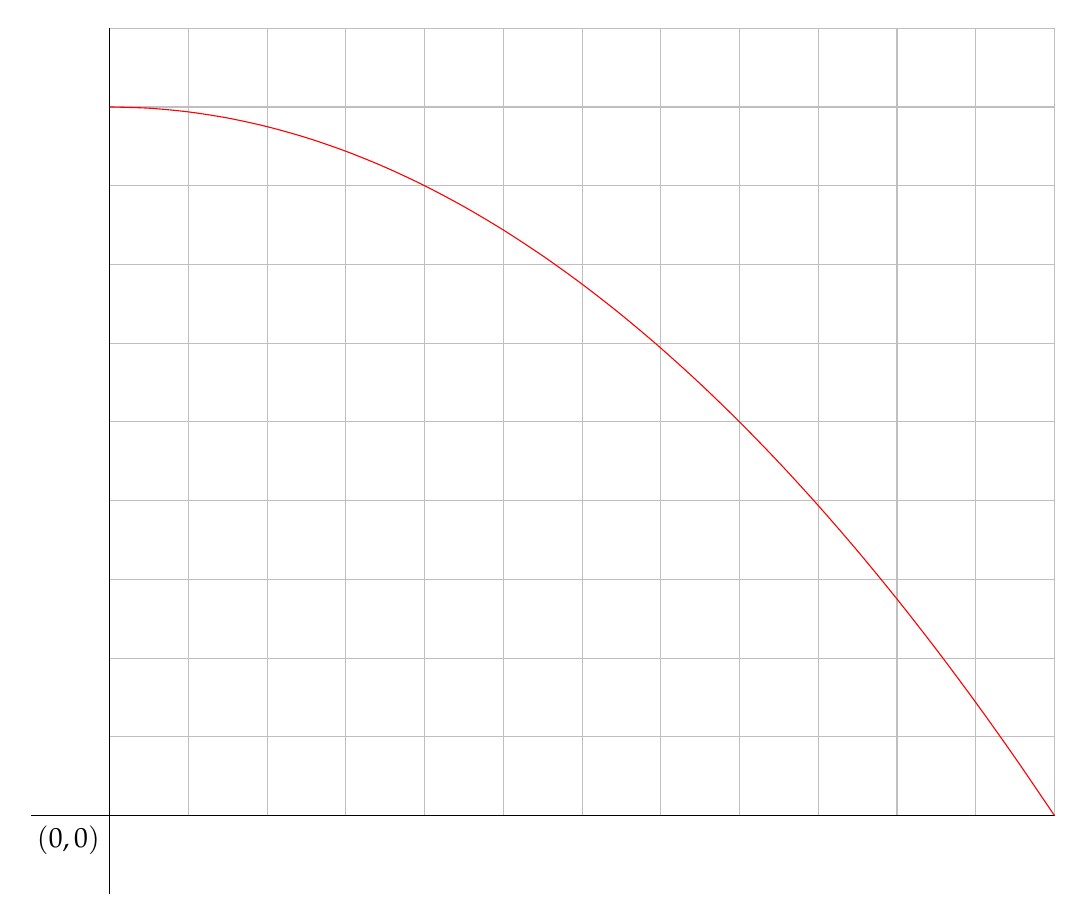
\begin{tikzpicture} [smooth]
   \draw [color=lightgray] (0,0) grid (12,10);
   \draw (-1,0) -- (12,0);
   \draw (0,-1) -- (0,0);
   \draw (0,0) node [anchor=north east] {$(0,0)$} -- (0,10);
   \draw [color=red, domain=0:12] plot (\x, {9-(\x/4)^2});
\end{tikzpicture}

\item A car accelerates from 0 to 40 mph in 30 seconds. The speedometer reading at each 5 second interval during this time is given in the table below. Estimate how far the car travels during this 30 second period using the velocities at:
\begin{enumerate}
\item The beginning of each time interval.
\item The end of each time interval.
\end{enumerate}

\begin{center}
\begin{tabular} {|c|c|c|c|c|c|c|c|}
\hline
{\bfseries t} (sec)&0&5&10&15&20&25&30\\
\hline
{\bfseries v} (mph)&0&6&14&23&30&36&40\\
\hline
\end{tabular}
\end{center}

\item Use Theorems 37 and 38 to justify the remaining property in Theorem 36: \[\int_a^b k\cdot f(x)\,dx =k\int_a^b f(x)\,dx\]

\item Use Theorems 37 and 38 to justify the remaining property in Theorem 39: If $f(x)\leq M$ for all $x$ in $[a,b]$, then \[\int_a^b f(x)\,dx\leq M(b-a).\]

\end{itemize}

\end{enumerate}

\end{document}
